\documentclass[a4paper,14pt]{extarticle} 
\usepackage[a4paper,top=1.5cm, bottom=1.5cm, left=2cm, right=1cm]{geometry}
%\usepackage[T2A]{fontenc}
%\usepackage[english, russian]{babel}
\usepackage{graphicx}
\graphicspath{{./pics/}}
\DeclareGraphicsExtensions{.pdf,.png,}

\usepackage{fontspec}
\setmainfont{Times New Roman}
\setsansfont{FreeSans}
\setmonofont{FreeMono}
\renewcommand{\baselinestretch}{1.5}
\usepackage{polyglossia}
\setdefaultlanguage{russian}
\setotherlanguages{english,russian}
\usepackage{setspace}
\usepackage[many]{tcolorbox}
\usepackage{array}

\begin{document}
    \begin{center}
        \thispagestyle{empty}
        \begin{singlespace}
        ФЕДЕРАЛЬНОЕ АГЕНТСТВО СВЯЗИ

        ФЕДЕРАЛЬНОЕ ГОСУДАРСТВЕННОЕ БЮДЖЕТНОЕ ОБРАЗОВАТЕЛЬНОЕ

        УЧРЕЖДЕНИЕ ВЫСШЕГО ОБРАЗОВАНИЯ

        «САНКТ-ПЕТЕРБУРГСКИЙ ГОСУДАРСТВЕННЫЙ УНИВЕРСИТЕТ ТЕЛЕКОММУНИКАЦИЙ ИМ. ПРОФ. М.А. БОНЧ-БРУЕВИЧА»

        (СПбГУТ)
        \end{singlespace}
        \vspace{-1ex}
        \rule{\textwidth}{0.4pt}
        \vspace{-5ex}

        \vspace{100px}
        \textbf{Лабораторная работа №3}\\
        Исследование свойств модели резисторного касакада с общим колектором в частотной и временной областях на ПК

    \vspace{100px}
    \end{center}
    \vspace{4ex}
    \begin{flushright}
    \parbox{12 cm}{
    \begin{flushleft}
        Выполнила бригада:\\
        Группа ИКТЗ-83\\
        \underline{Громов А.А., Миколаени М.С., Мазеин Д.С.} \hfill \rule[-0.85ex]{0.09\textwidth}{0.6pt}\\
        \vspace{-1ex}
        \footnotesize \textit{ (Ф.И.О., № группы) \hfill (подпись)} \normalsize


    \end{flushleft}
    }
    \end{flushright}
    \begin{center}
        \vfill
        Санкт-Петербург

        2020

    \end{center}
    \newpage

    \textbf{Цель работы:} Изучить свойства усилительного каскада с общим коллектором (ОК) в режиме малого сигнала. Выполнить анализ в частотной и временной областях. Исследовать свойства каскада при изменении сопротивлений источника сигнала, нагрузки и элементов схемы. Определить входное и выходное сопротивления каскада.

    \textbf{Пункт 1:}
    \begin{center}
        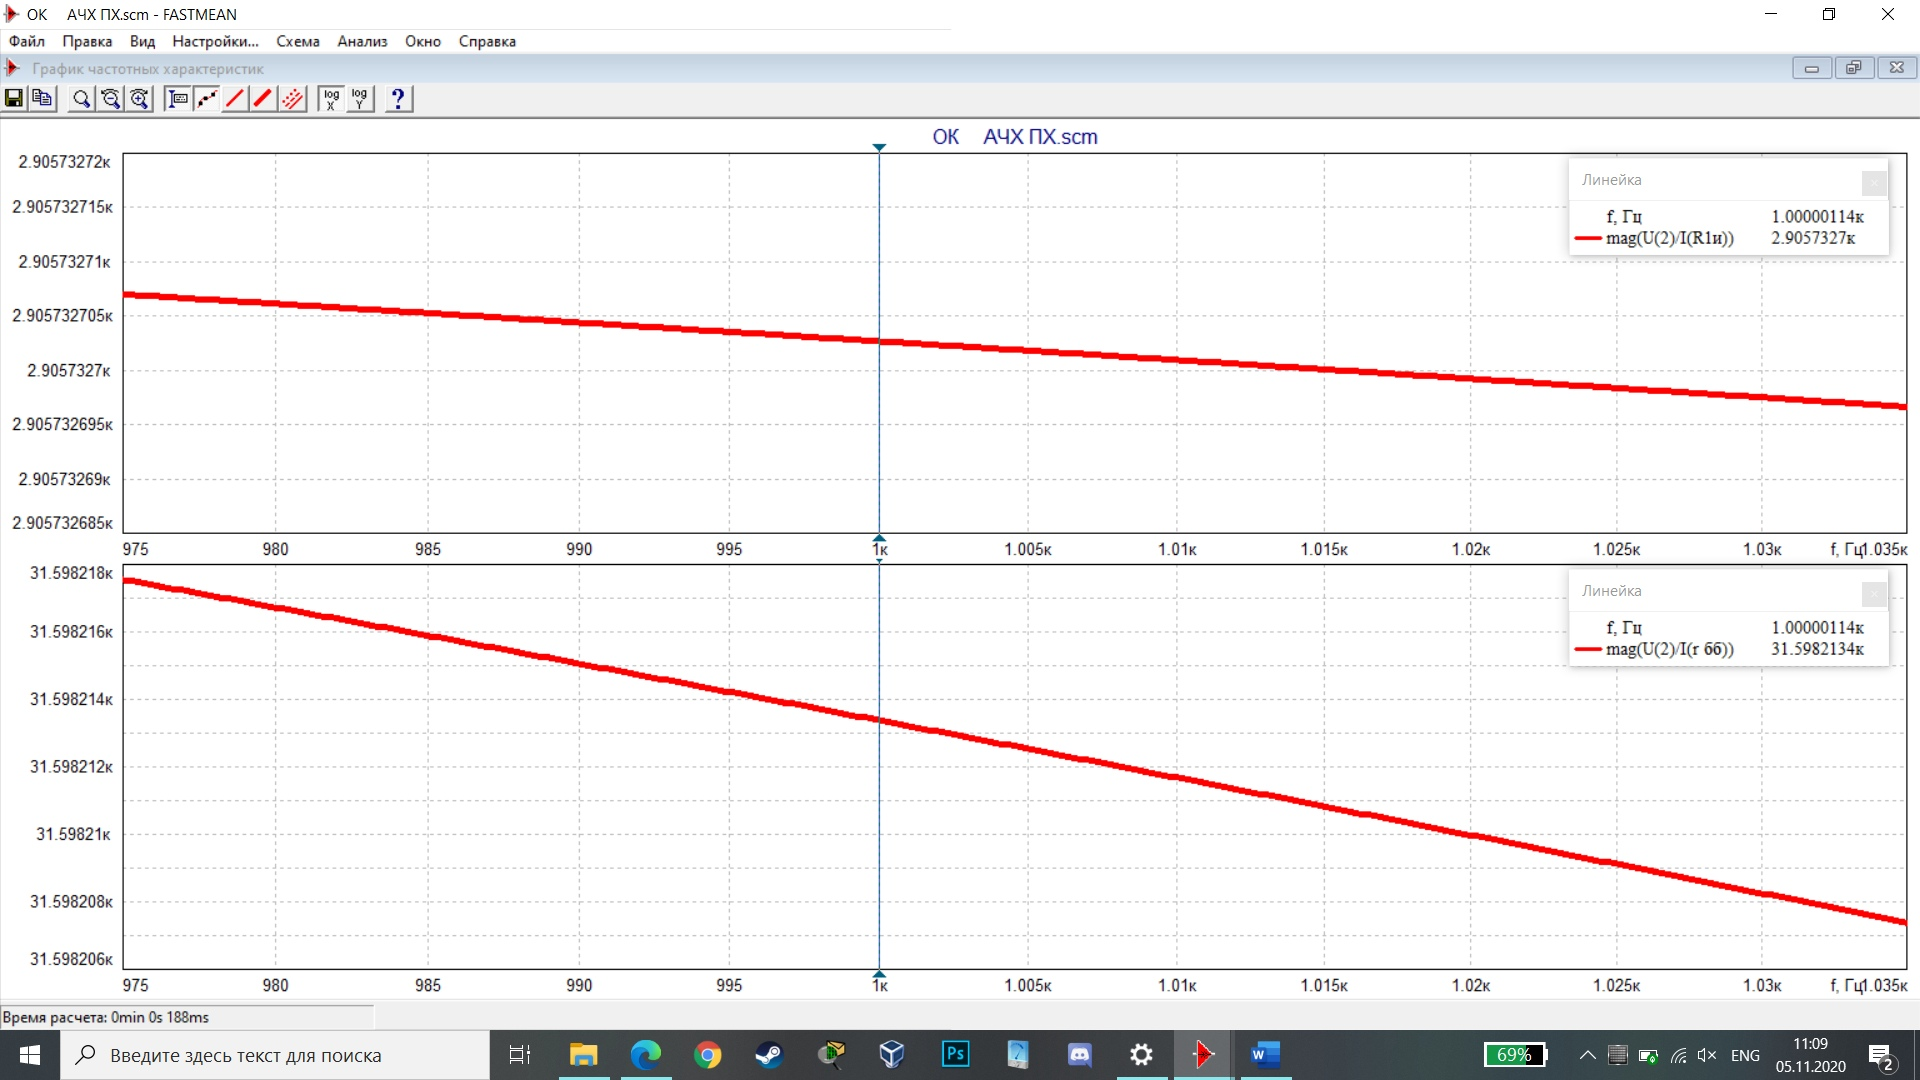
\includegraphics[scale=0.25]{1.jpg}
    \end{center}

    Окно измерения входного сопротивления 
    \begin{table}[ht]
        \begin{center}
            \caption{Измерение входного сопротивления каскада с ОК}
            \begin{tabular}{ |c|c| }
                \hline
                Измерение & Величина входного сопротивления, КОм\\
                \hline
                с учётом сопротивления $R_{\text{б}}$ & 31.6\\
                \hline
                без учёта сопротивления $R_{\text{б}}$ & 2.91\\
                \hline
            \end{tabular}
        \end{center}
    \end{table}

    \newpage
    \textbf{Пункт 2:}
    \begin{center}
        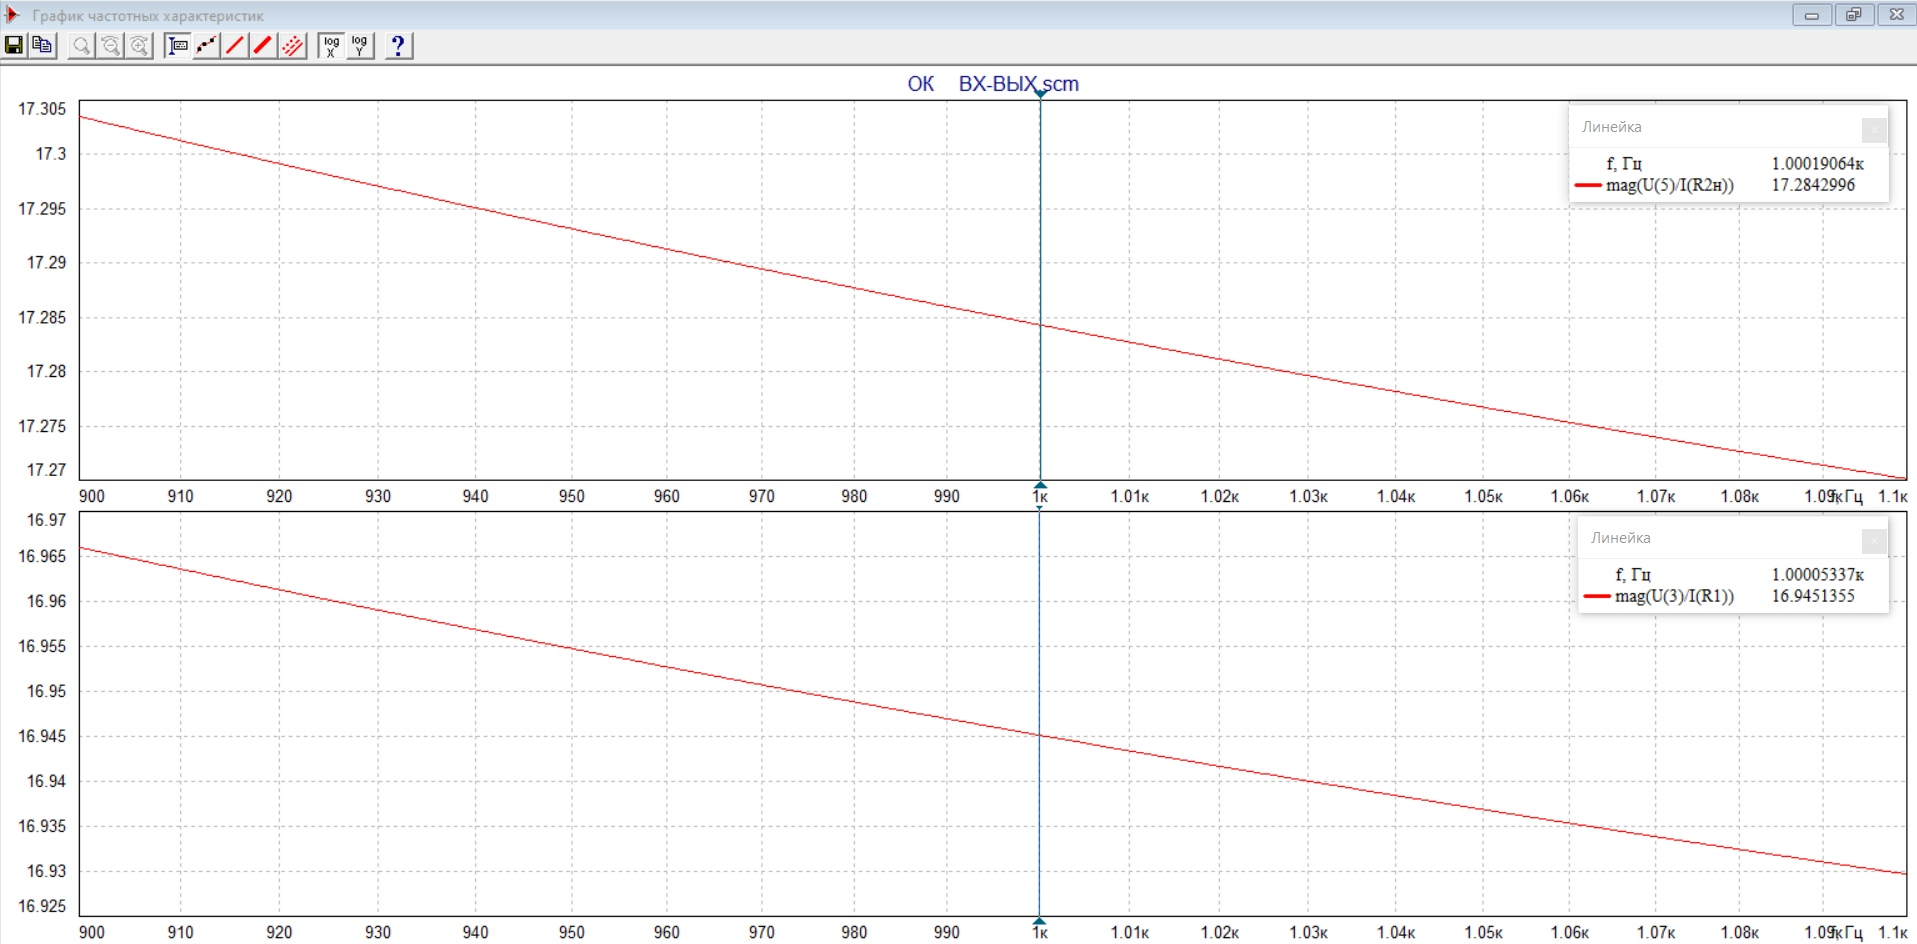
\includegraphics[scale=0.25]{2.jpg}
    \end{center}

    Выходное сопротивление с учетом $R_{\text{э}}$ 17.29Ом

    Выходное сопротивление без учета $R_{\text{э}}$ 16.95Ом

    \textbf{Выводы по пункту 2:}
    \vspace{-6ex}
    \begin{singlespace}
        \begin{itemize}
            \item Входное сопротивление каскада с ОК примерно на 3 порядка больше, чем выходное.
        \end{itemize}
    \end{singlespace}

    \newpage 
    \textbf{Пункт 3:}
    \begin{center}
        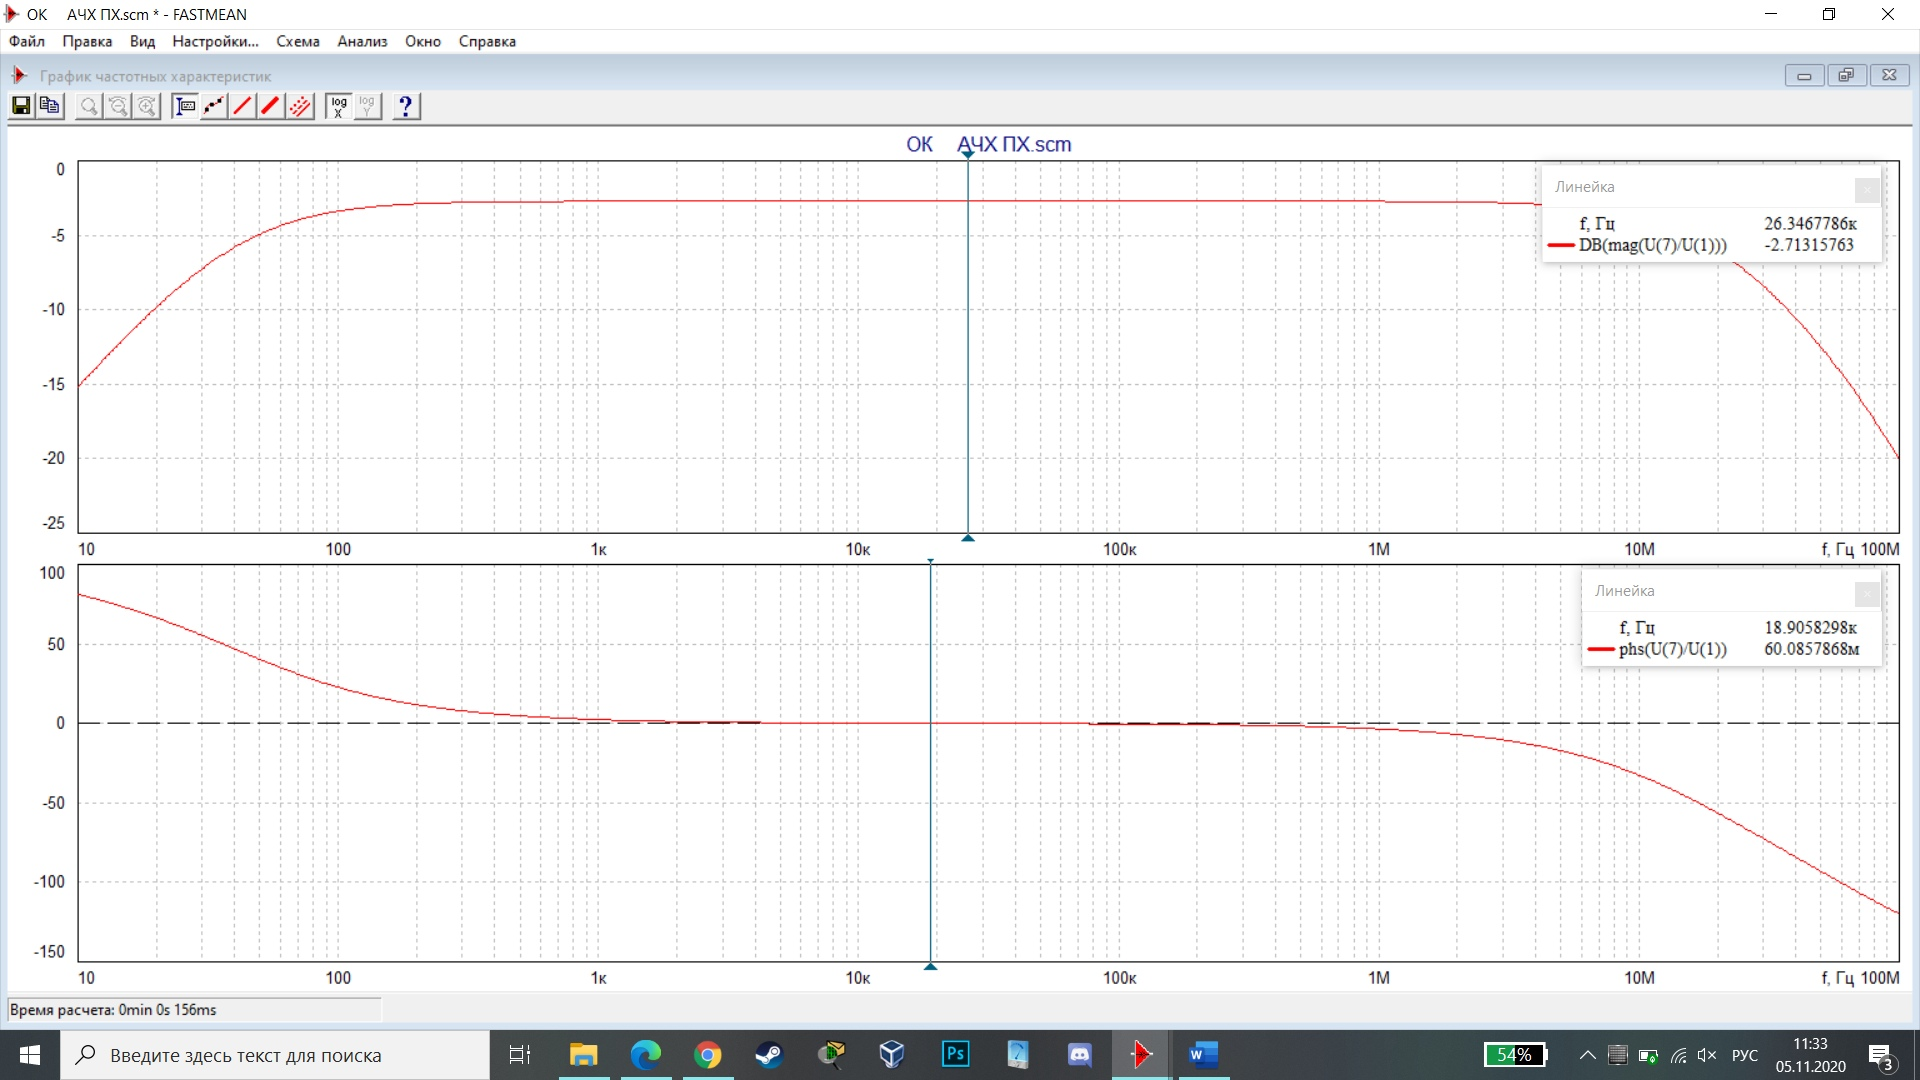
\includegraphics[scale=0.25]{3.1.jpg}
    \end{center}
    \begin{center}
        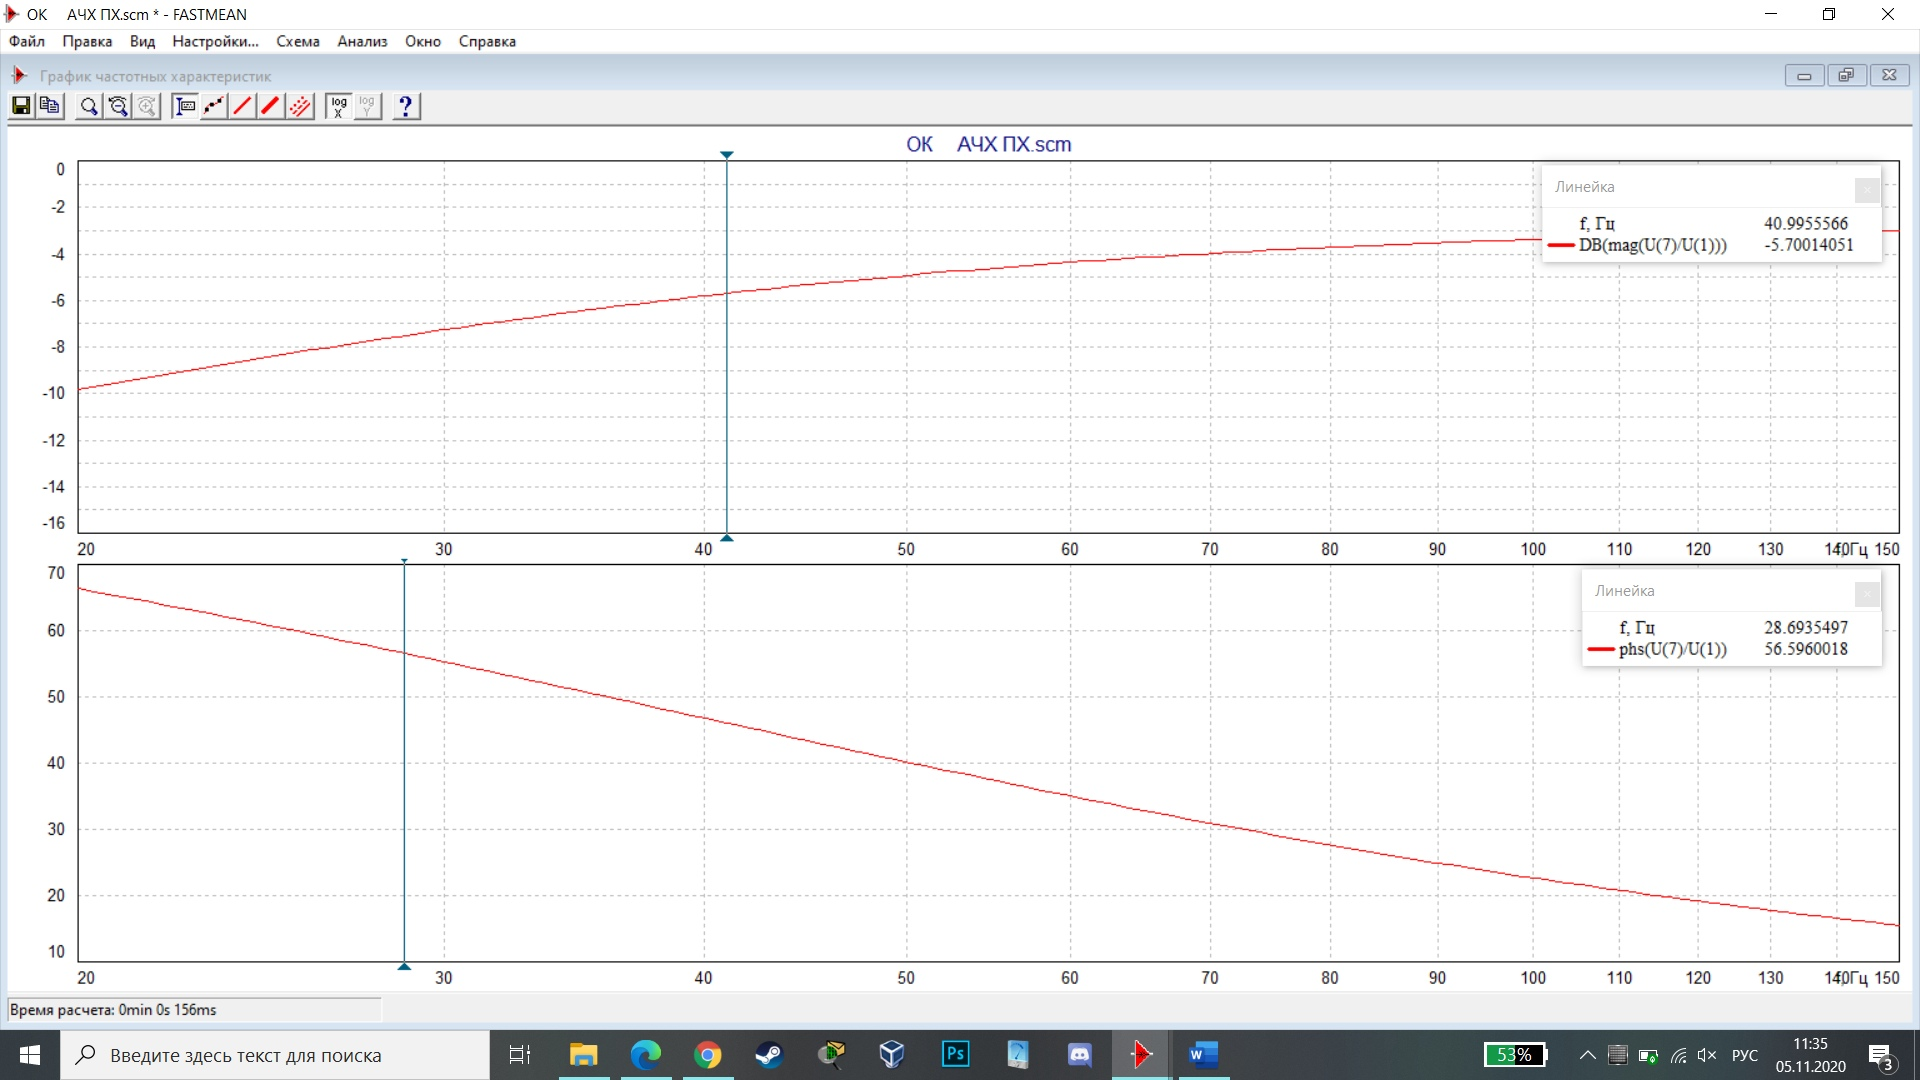
\includegraphics[scale=0.25]{3.2.jpg}
    \end{center}
    \begin{center}
        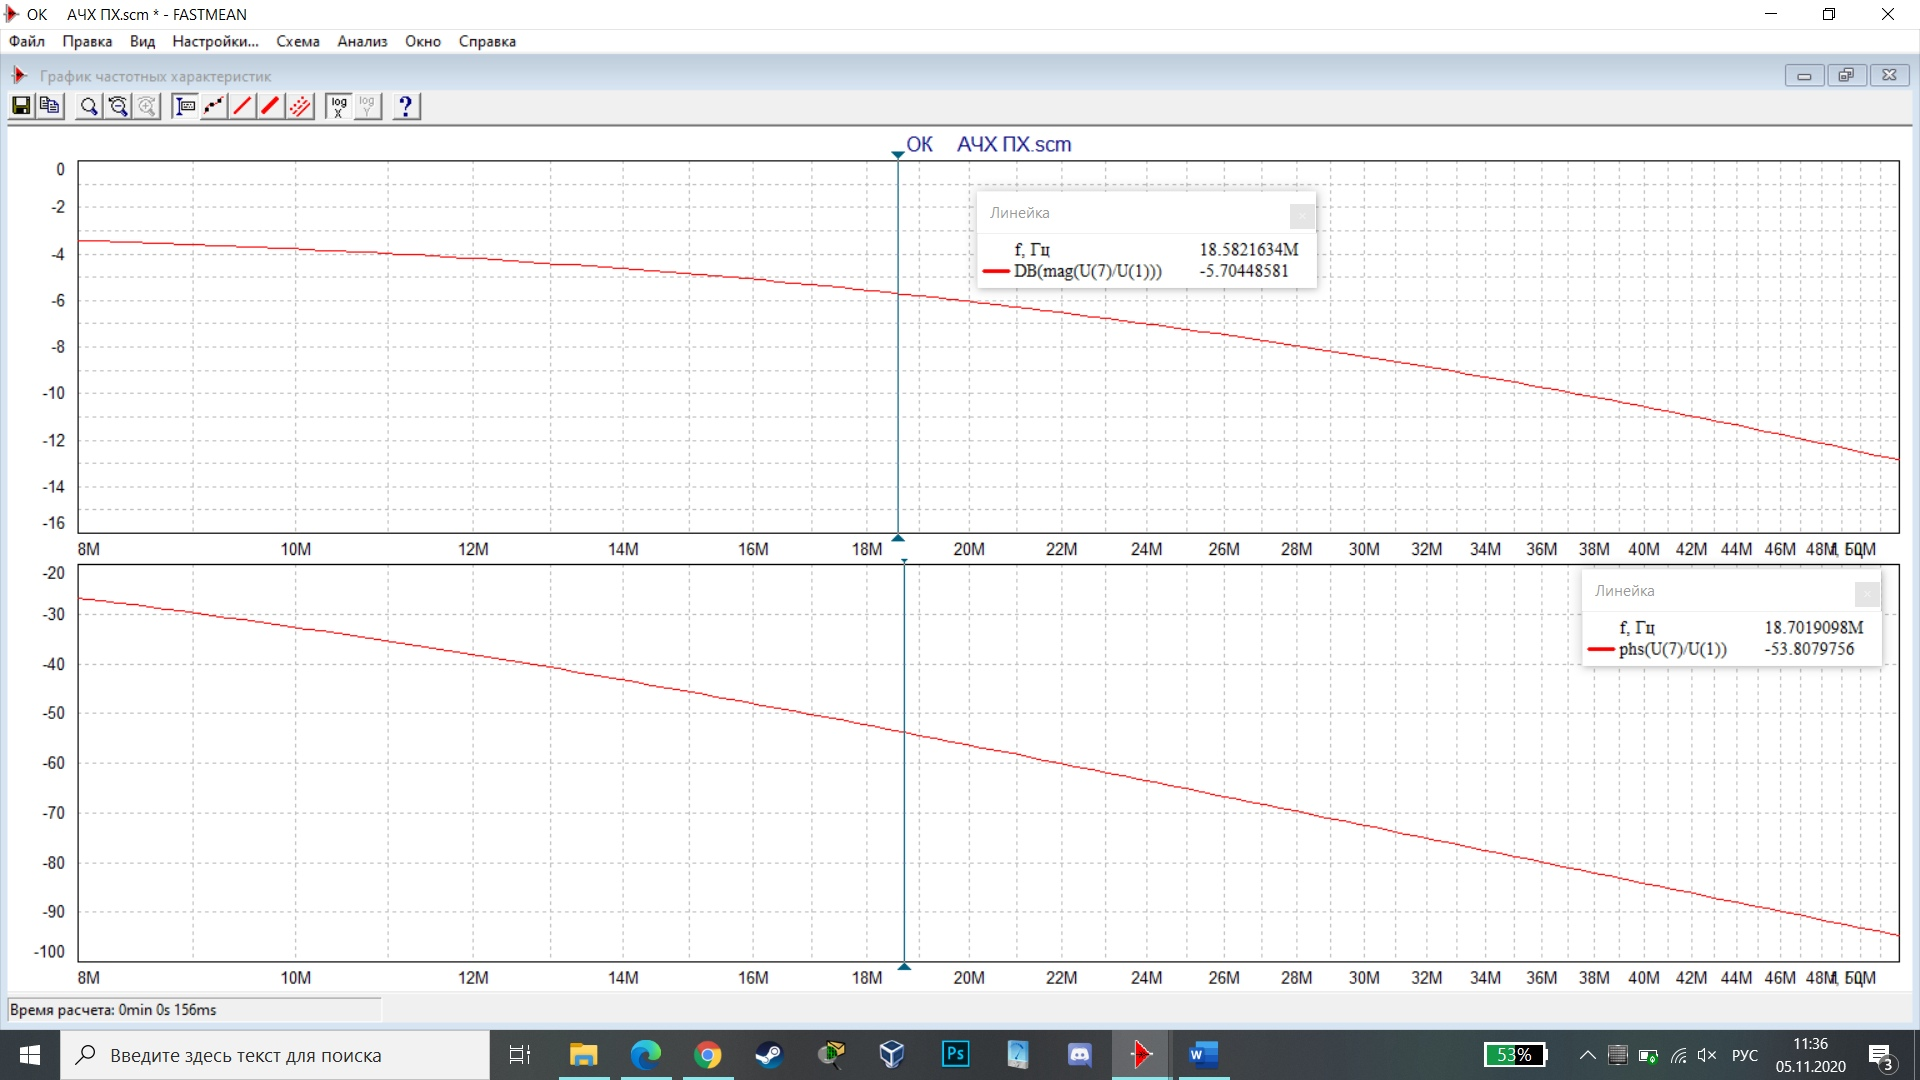
\includegraphics[scale=0.25]{3.3.jpg}
    \end{center}

    \begin{table}[ht]
        \begin{center}
            \caption{Измерение АЧХ каскада с ОК}
            \begin{tabular}{ |c|c|c|c|c| }
                \hline
                $K_{\text{скв}}$, Дб & ($K_{\text{скв}}$ - 3), Дб&fн, Гц & fв, МГц & ∆f=fв−fн, МГц \\
                \hline 
                -2.7 & -5.7 & 41 & 18.6 & 18.56\\
                \hline
            \end{tabular}\\
        \end{center}
    \end{table}
    \textbf{Выводы по пункту 3:}
    \vspace{-6ex}
    \begin{singlespace}
        \begin{itemize}
            \item Схема с ОК не инвертирует входной сигнал.
            \item У схемы каскада с ОК рабочая полоса частот больше, чем у схемы с ОЭ.
            \item Схема каскада с ОК, в отличие от схемы касакада с ОЭ, ослабляет сигнал. 
        \end{itemize}
    \end{singlespace}


    \newpage
    \textbf{Пункт 4:}

    \begin{table}[ht]
        \begin{center}
            \caption{Измерение ПХ каскада с ОК}
            \begin{tabular}{|>{\centering}m{5cm}|>{\centering}m{5.5cm}|>{\centering}m{5cm}|}
                \hline 
                Время импульса & $t_{\text{и}}$= 25 мкс & $t_{\text{и}}$=1.25 мс
                \tabularnewline
                \hline
                Частота f, Гц & 20000 & 400
                \tabularnewline
                \hline 
                Осциллограмма импульса & \vspace{0.5cm}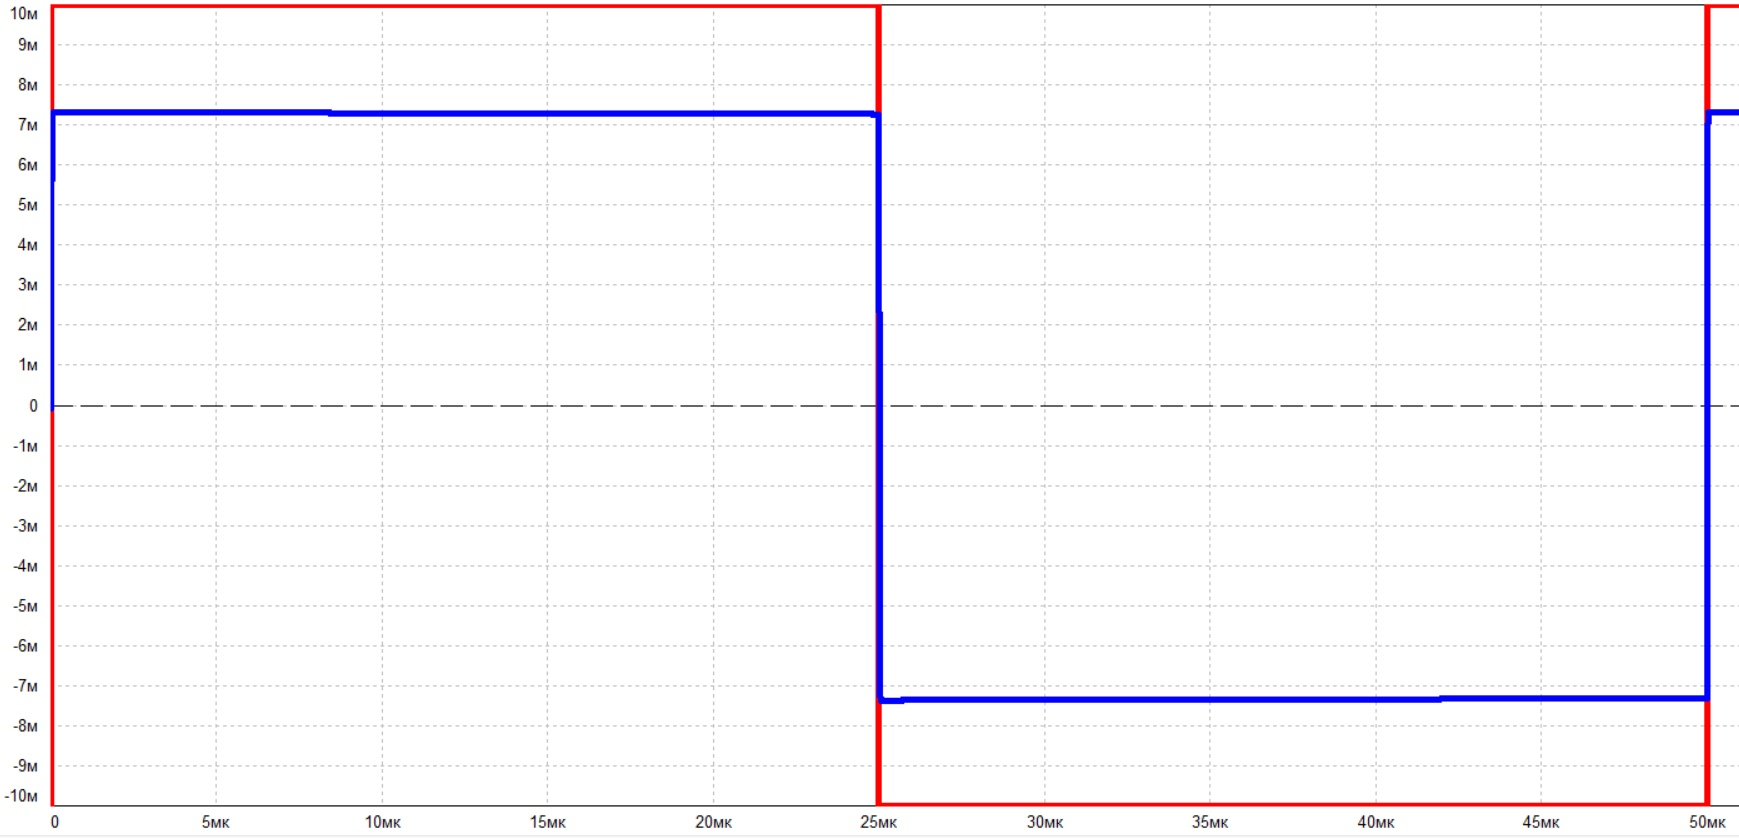
\includegraphics[scale=0.089]{4.1.jpg} & \vspace{0.5cm}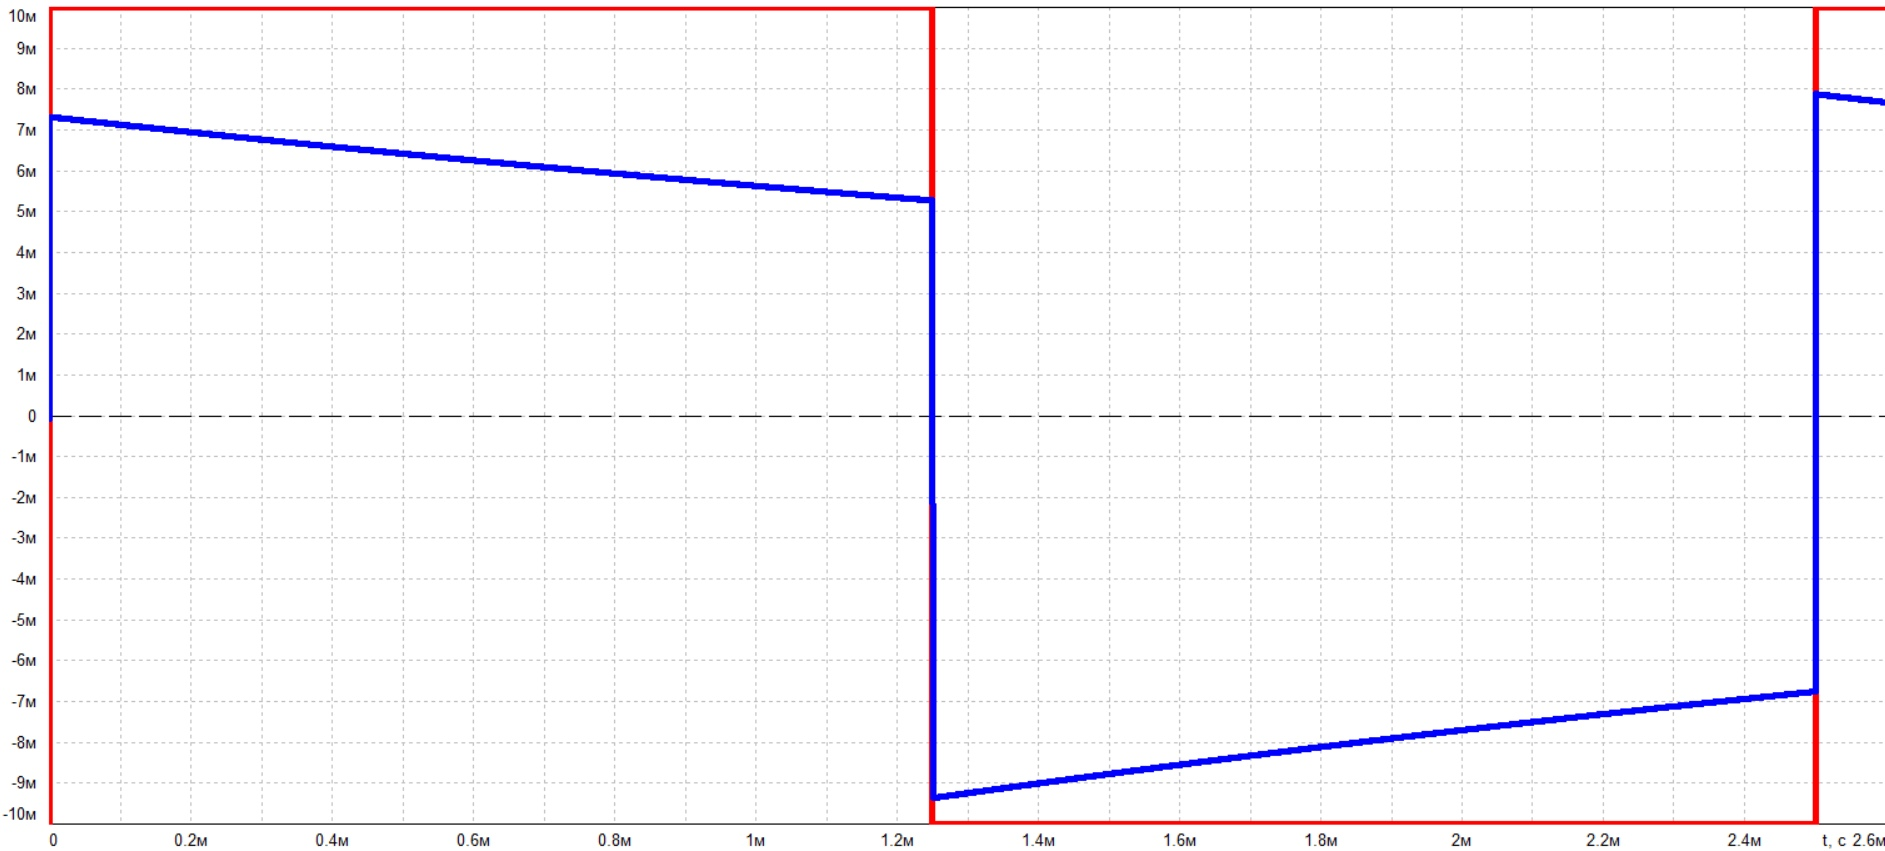
\includegraphics[scale=0.075]{4.2.jpg}
                \tabularnewline
                \hline 
                \parbox[c][3cm]{5cm}{Измеренный спад вершины импульса ∆, \% \\$∆=\frac{U_{\text{уст}}-U_{\text{вых}}}{U_{\text{уст}}} \cdot 100\%$}& - & 27.9
                \tabularnewline
                \hline 
                Рассчитанный спад вершины импульса ∆, \% & 0.62 & 31.4 
                \tabularnewline
                \hline 
                Осциллограмма увеличенной области нарастания импульса & \vspace{0.5cm}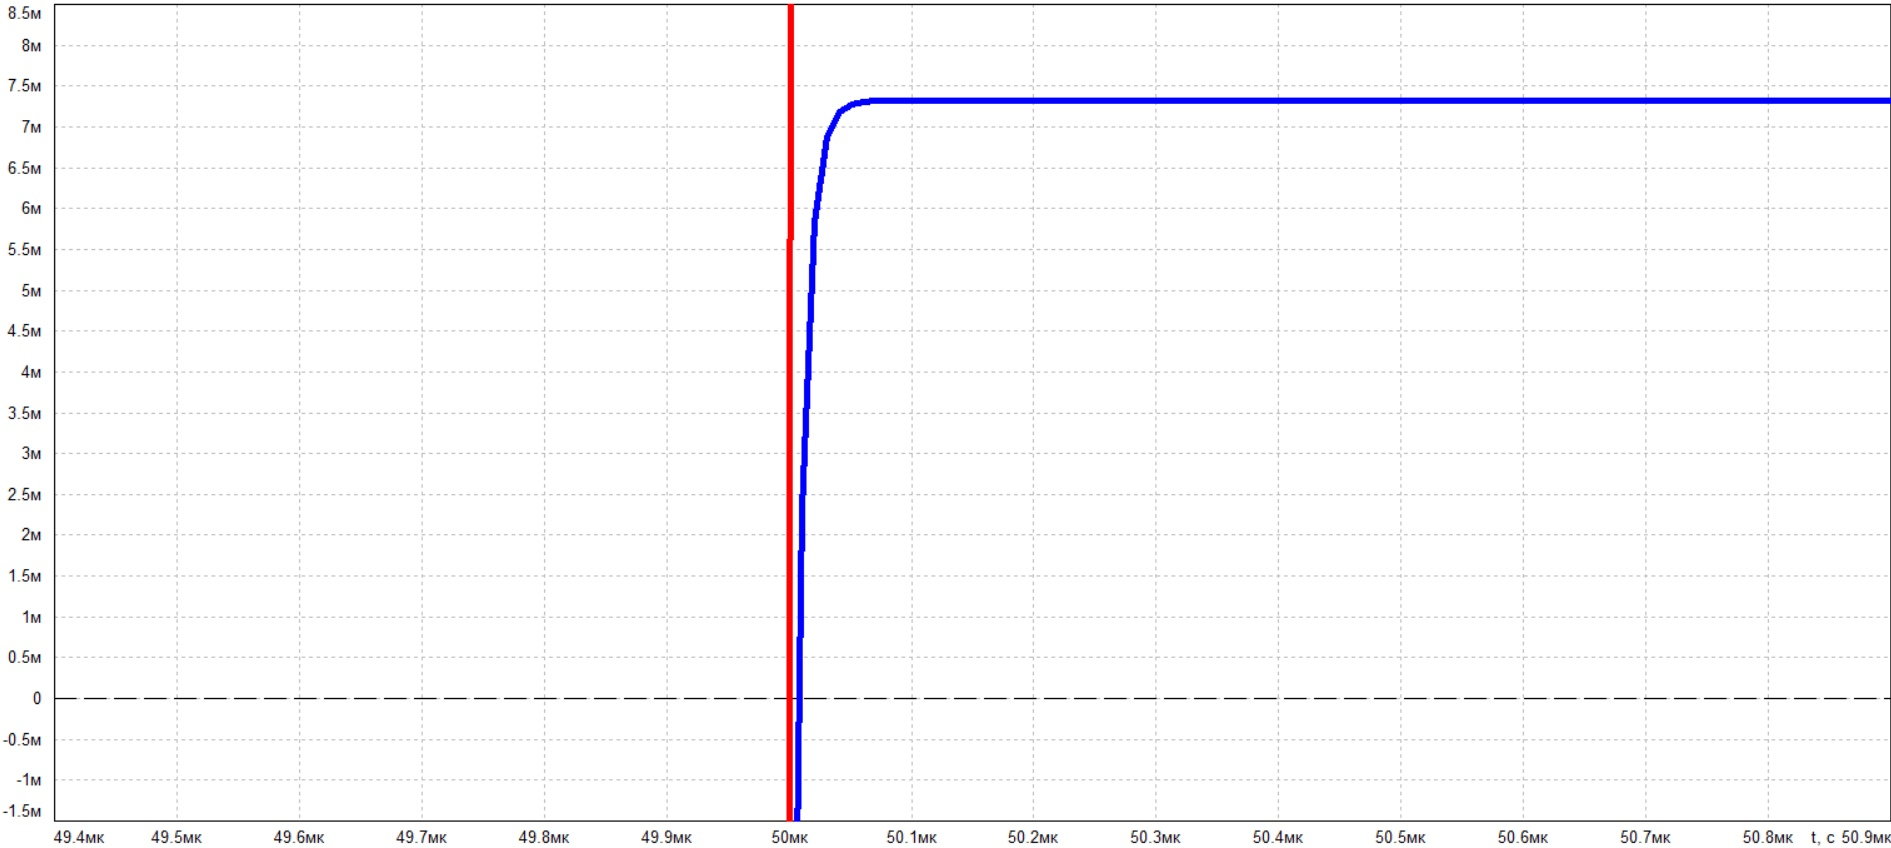
\includegraphics[scale=0.075]{4.4.jpg} & \vspace{0.5cm}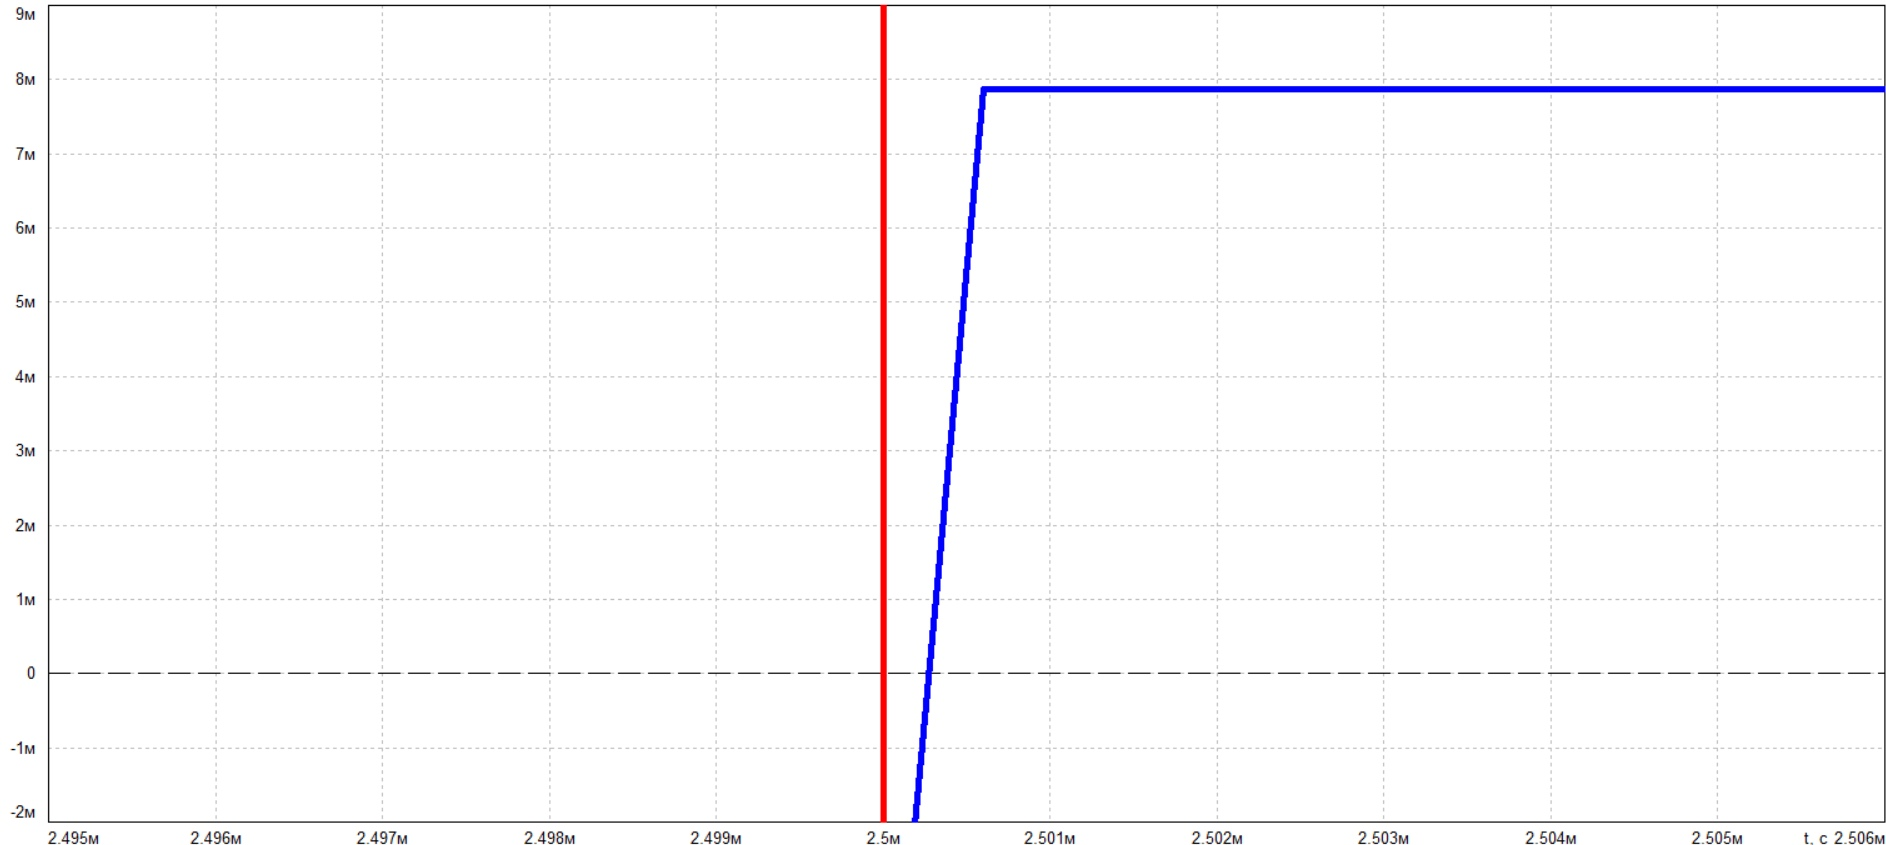
\includegraphics[scale=0.075]{4.3.jpg} 
                \tabularnewline
                \hline 
                \parbox[c][3cm]{5cm}{Измеренное время нарастания импульса \\ $t_{\text{Н}}$ = $t_{\text{2}}$ – $t_{\text{1}}$, нс} & 19.12 & - 
                \tabularnewline
                \hline 
                Рассчитанное время нарастания импульса $t_{\text{н}}$, нс & 18.8 & 18.8
                \tabularnewline
                \hline 
            \end{tabular}
        \end{center}
    \end{table}

    \textbf{Выводы по пункту 4:}
    \vspace{-6ex}
    \begin{singlespace}
        \begin{itemize}
            \item Измеренный спад вершины импульса практически совпадает с рассчитанным спадом вершины импульса;
            \item Измеренное время нарастания импульса практически совпадает с рассчитанное временем нарастания импульса;
        \end{itemize}
    \end{singlespace}

    \newpage
    \textbf{Пункт 5}
    \begin{table}[ht]
        \begin{center}
            \caption{Оценка влияния параметров схемы на ПХ и АЧХ}
            \begin{tabular}{|c|c|c|c|c|c|c|c|}
                \hline 
                № & $R_1$ & $R_2$ & $K_{\text{скв}}$ & $f_{\text{н}}$ & $f_{\text{в}}$ & \parbox[c]{4cm}{\begin{center}∆ \\при $t_{\text{и}}$= 25 мкс \end{center}} & \parbox[c]{4cm}{\begin{center}$t_{n}$ \\при $t_{\text{и}}$= 1.25 мс \end{center}}
                \tabularnewline
                \hline 
                п/п & кОм & кОм & дБ & Гц & МГц & \% & нс
                \tabularnewline
                \hline 
                1 & 1 & 3,6 & -2,7 & 41 & 18,6 & 27.9 & 19.12
                \tabularnewline
                \hline 
                2 & 1 & 10 & -2,7 & 41 & 18,6 & 27.2 & 19.3
                \tabularnewline
                \hline        
                3 & 5 & 3,6 & -8.8 & 13.8 & 11 & 15 & 46.44
                \tabularnewline
                \hline        
                4 & 5 & 10 & -8,8 & 13,6 & 11,1 & 13.8 & 46.67 
                \tabularnewline
                \hline        
            \end{tabular}
        \end{center}
    \end{table}

    \begin{center}
        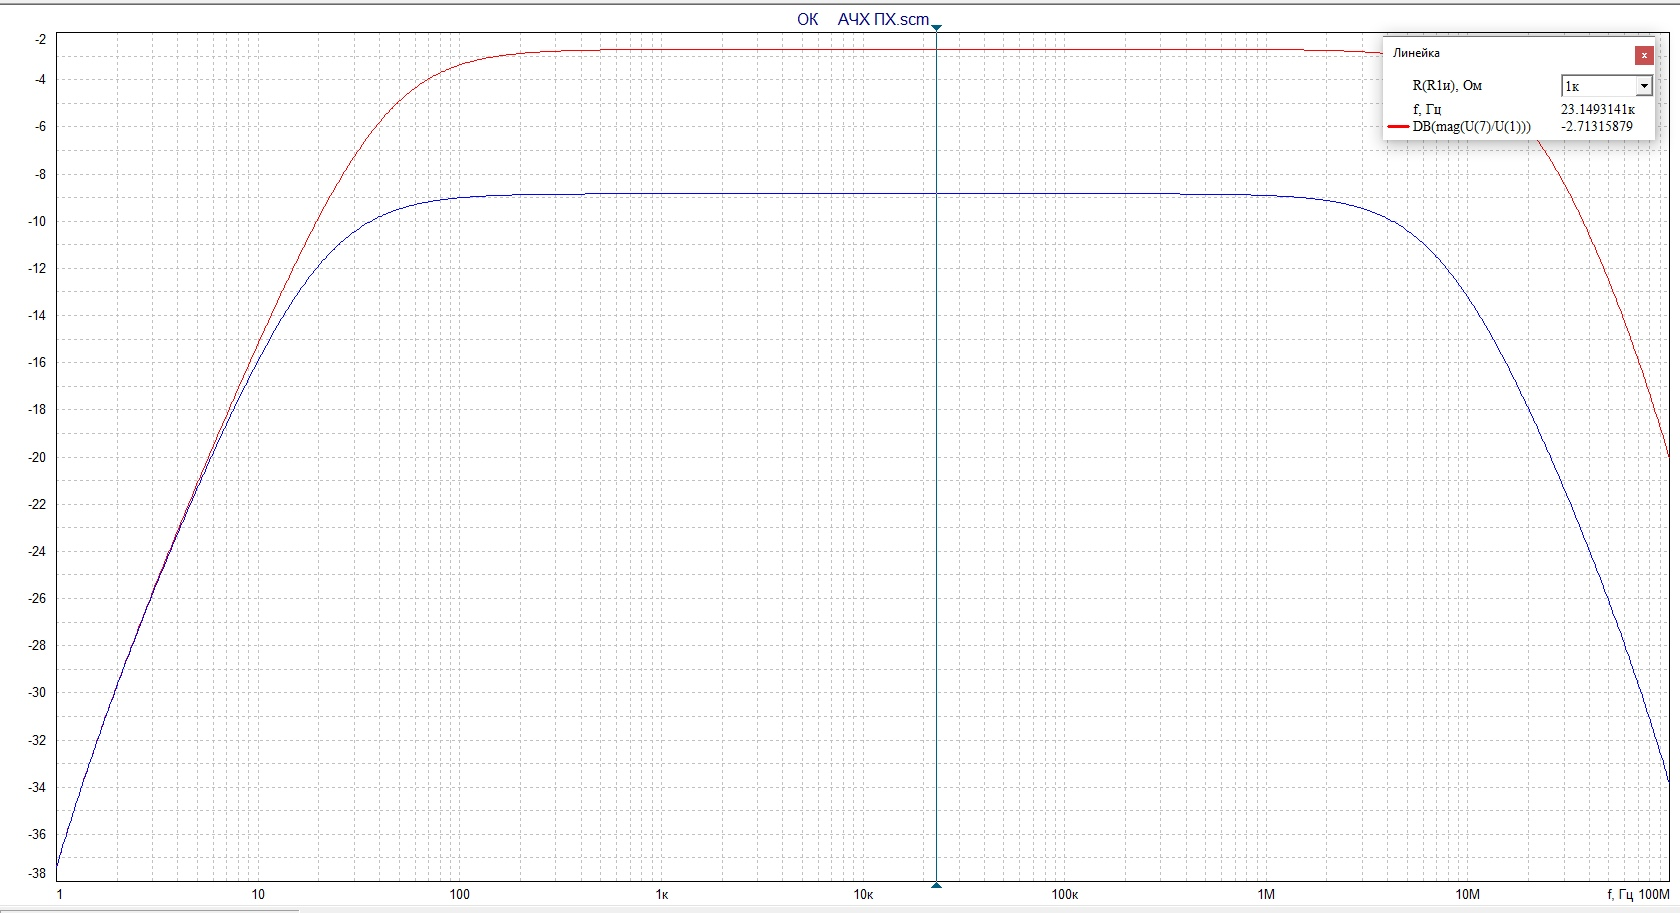
\includegraphics[scale=0.3]{5.5.jpg}
    \end{center}

    АЧХ при $R_2$ = 3.6кОм

    \begin{center}
        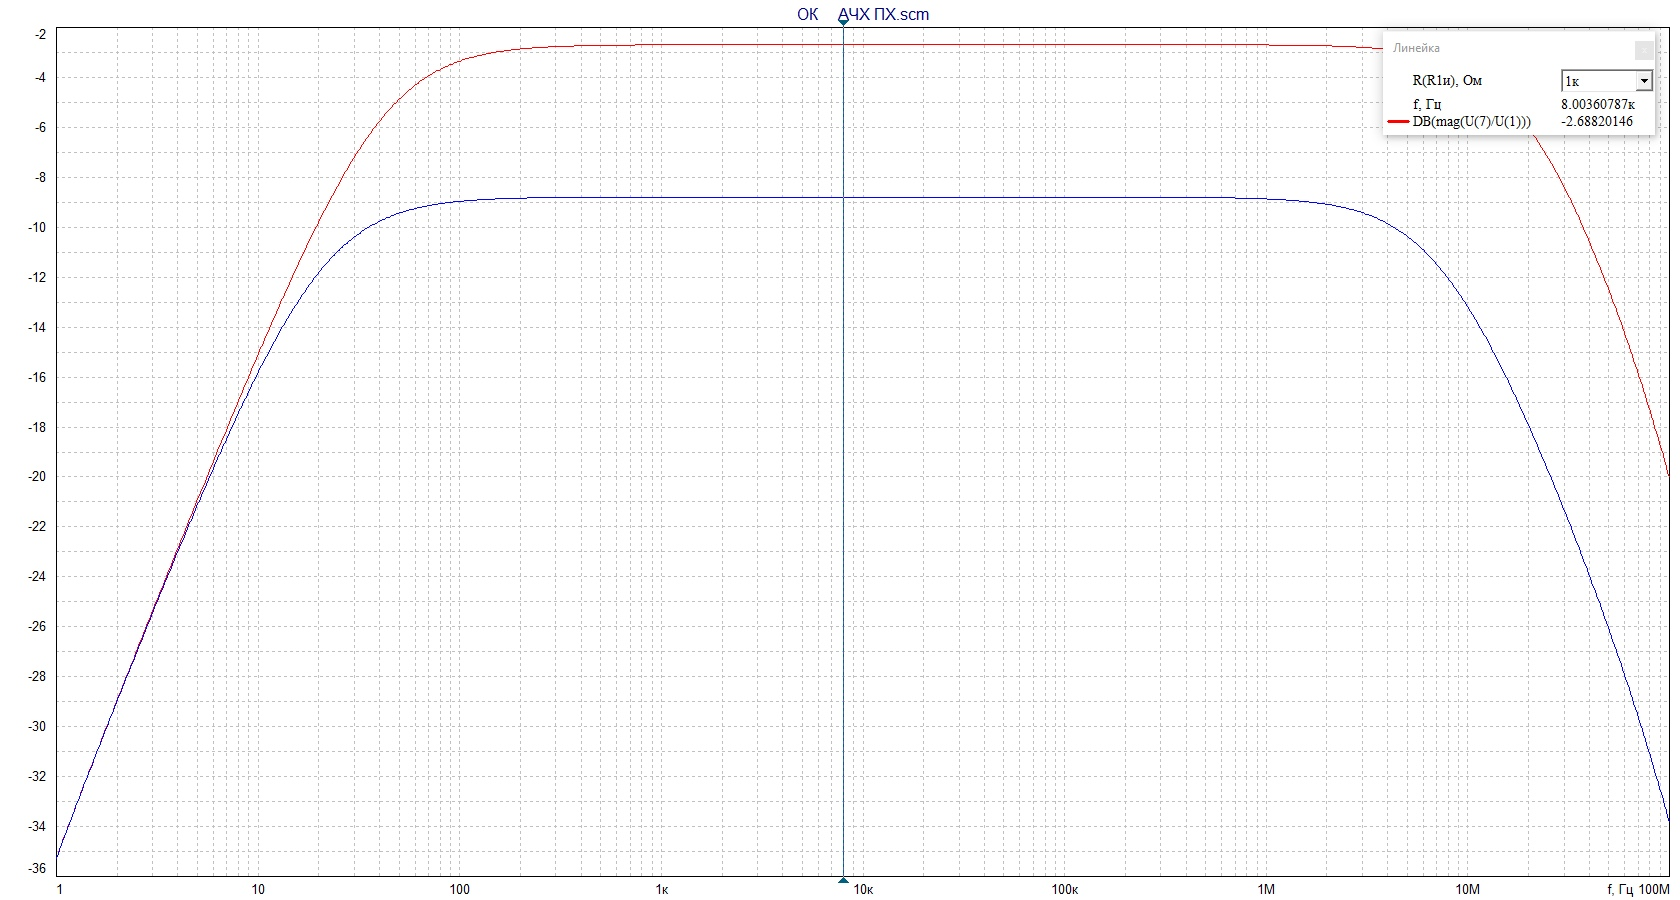
\includegraphics[scale=0.3]{5.6.jpg}
    \end{center}

    АЧХ при $R_2$ = 10кОм

    \begin{center}
        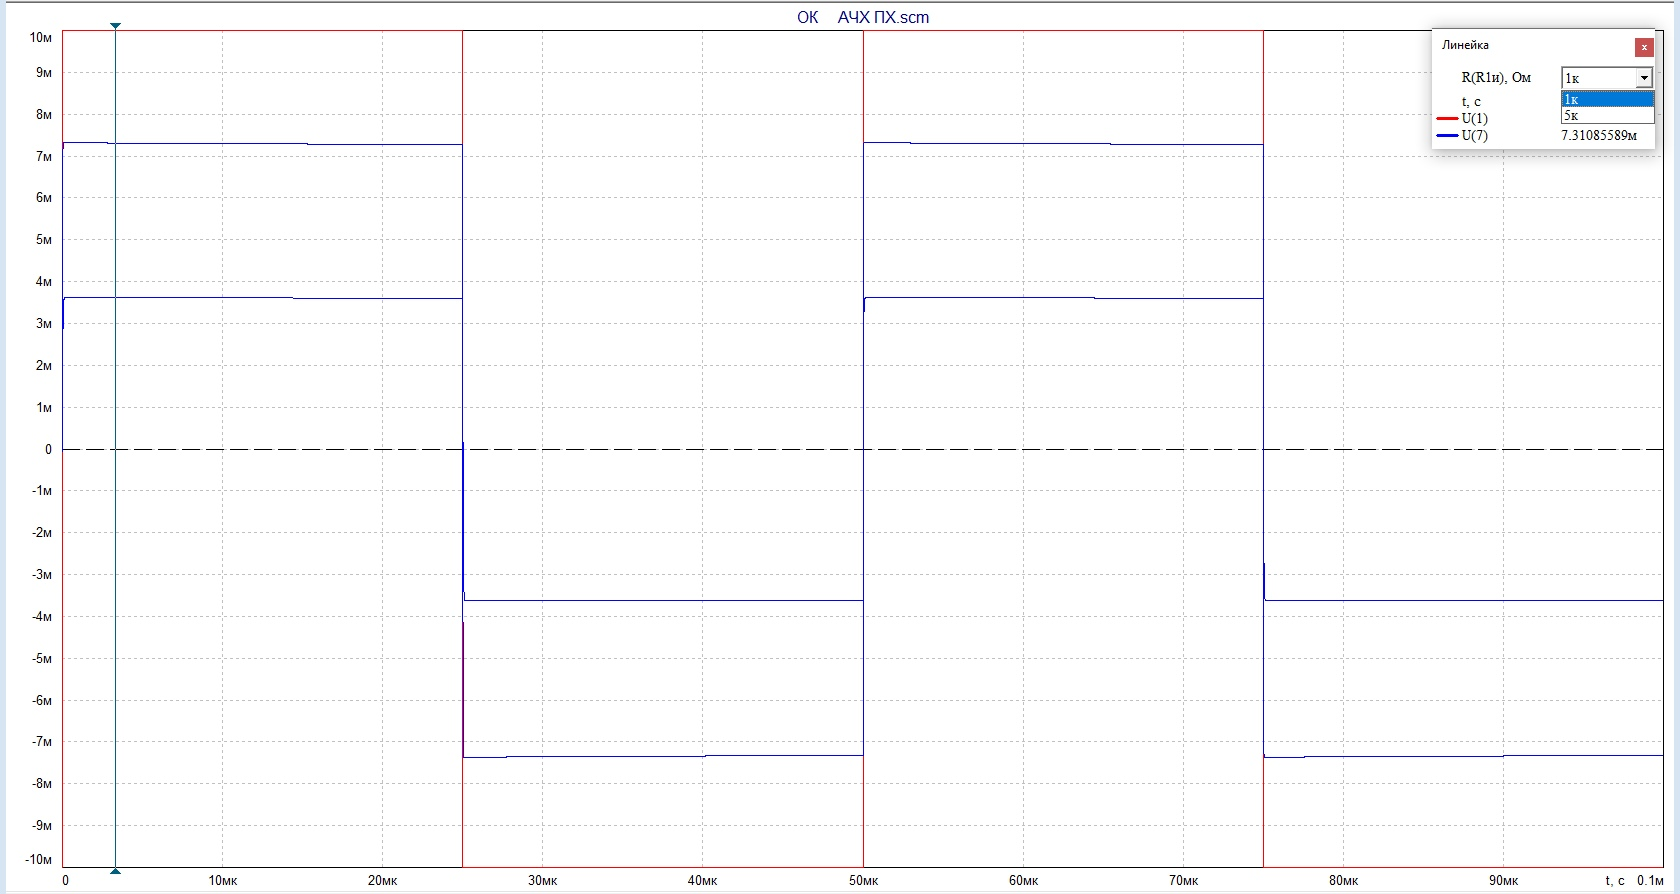
\includegraphics[scale=0.3]{5.1.jpg}
    \end{center}

    ПФ при $R_2$ = 3.6кОм, f = 20кГц

    \begin{center}
        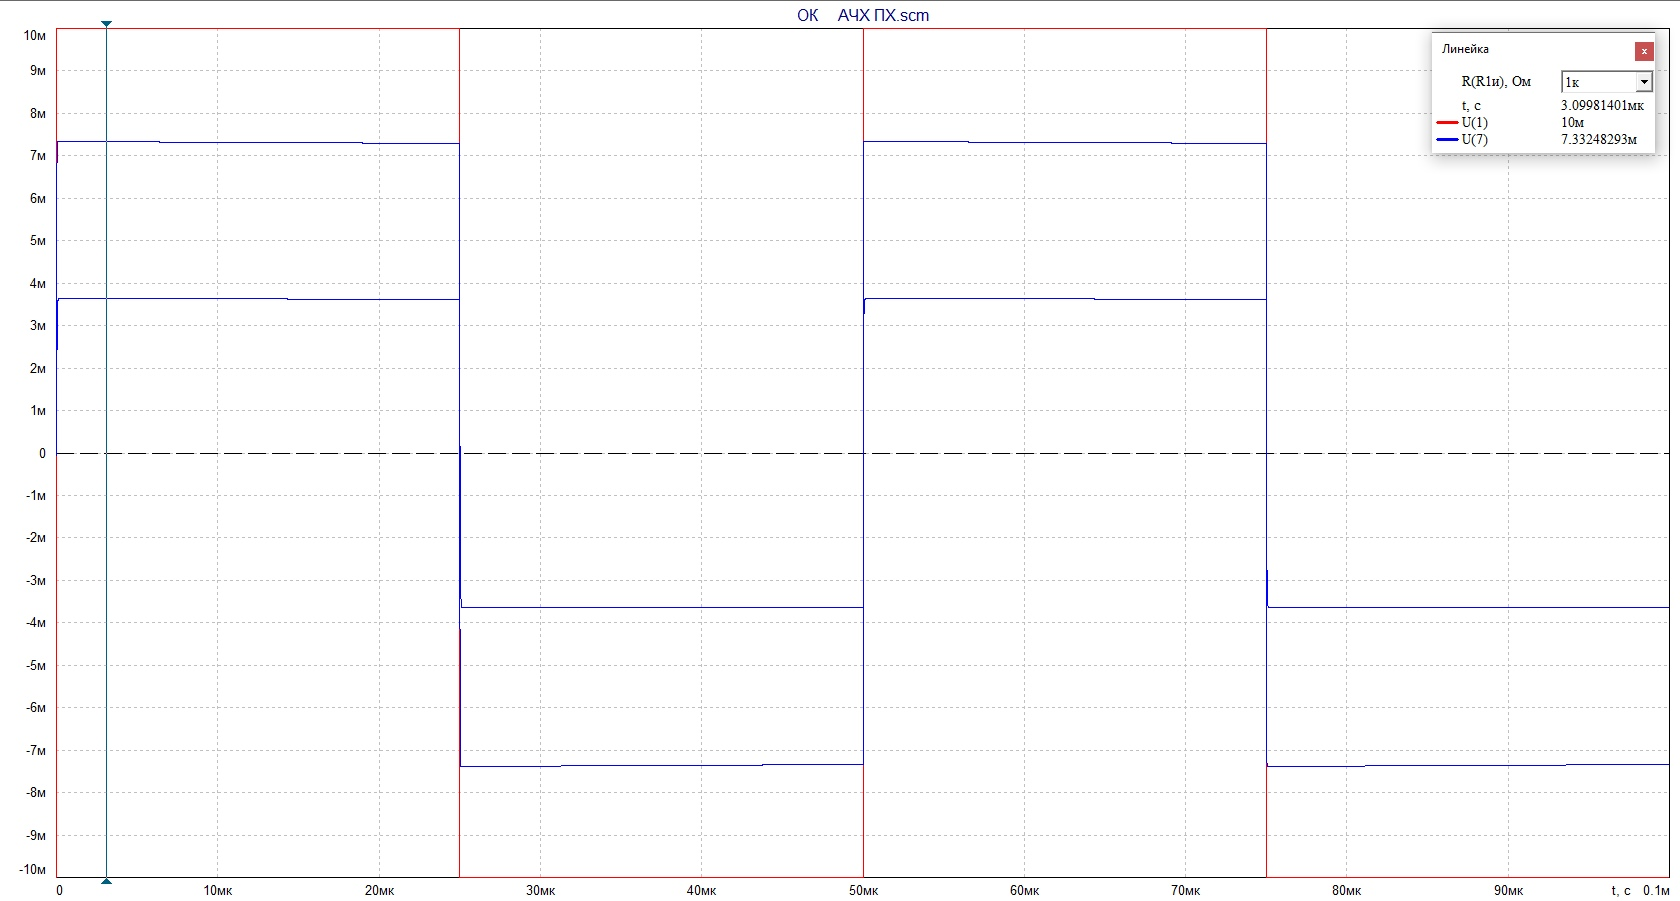
\includegraphics[scale=0.3]{5.2.jpg}
    \end{center}

    ПФ при $R_2$ = 10ОкОм, f=20кГц

    \begin{center}
        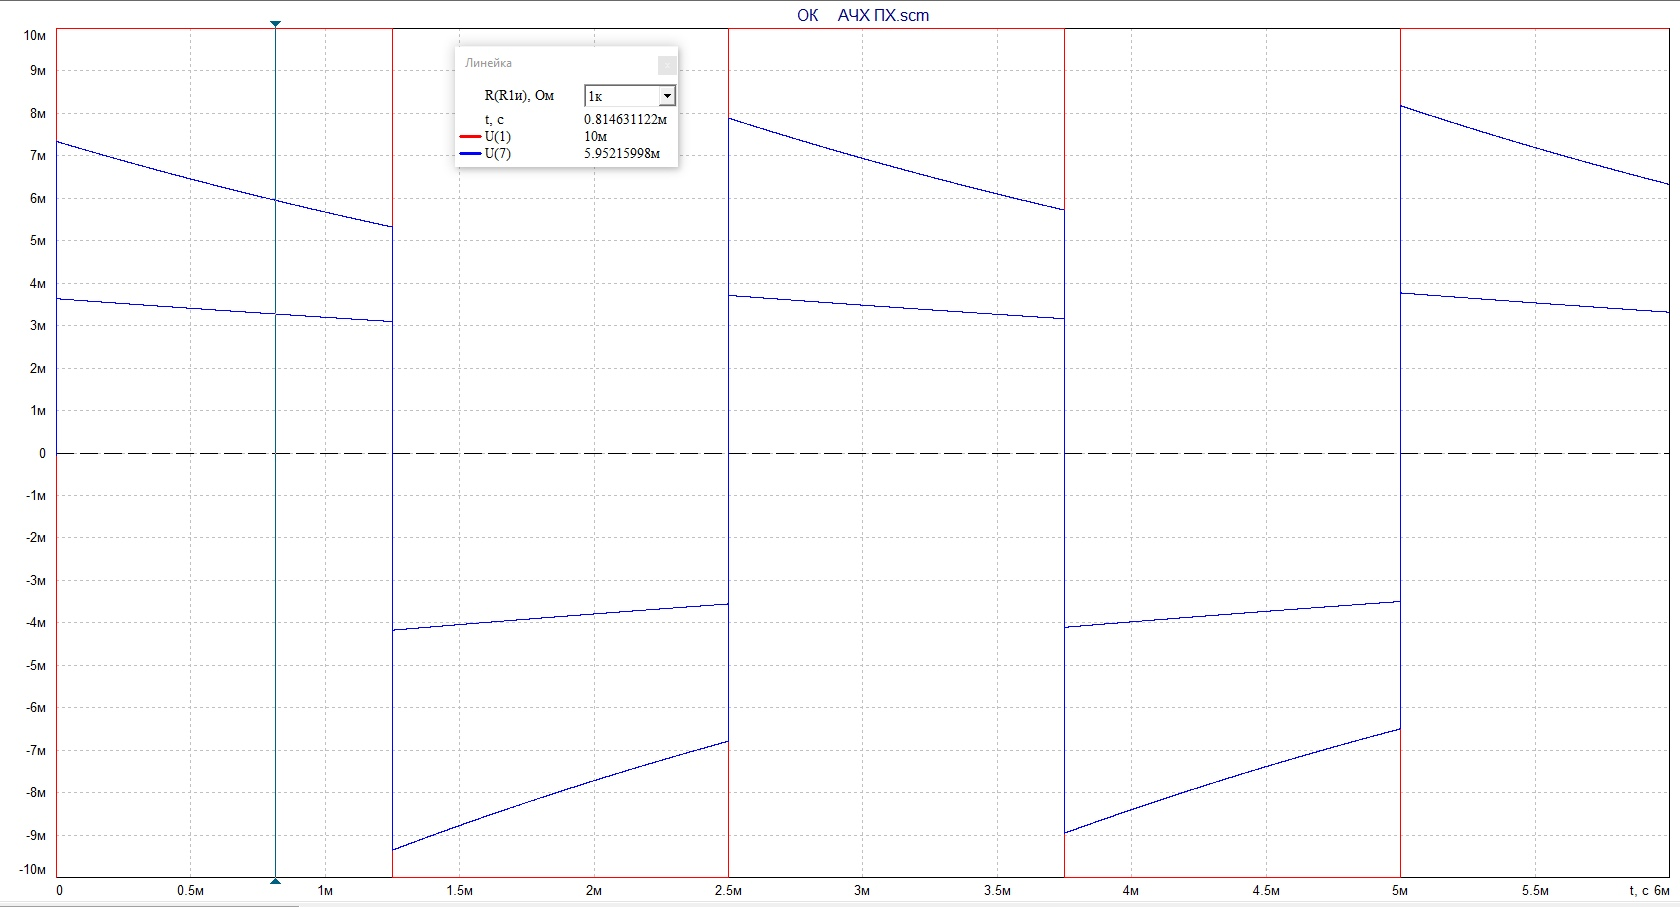
\includegraphics[scale=0.3]{5.3.jpg}
    \end{center}
    
    ПФ при f = 400Гц, $R_2$ = 10кОм 

    \begin{center}
        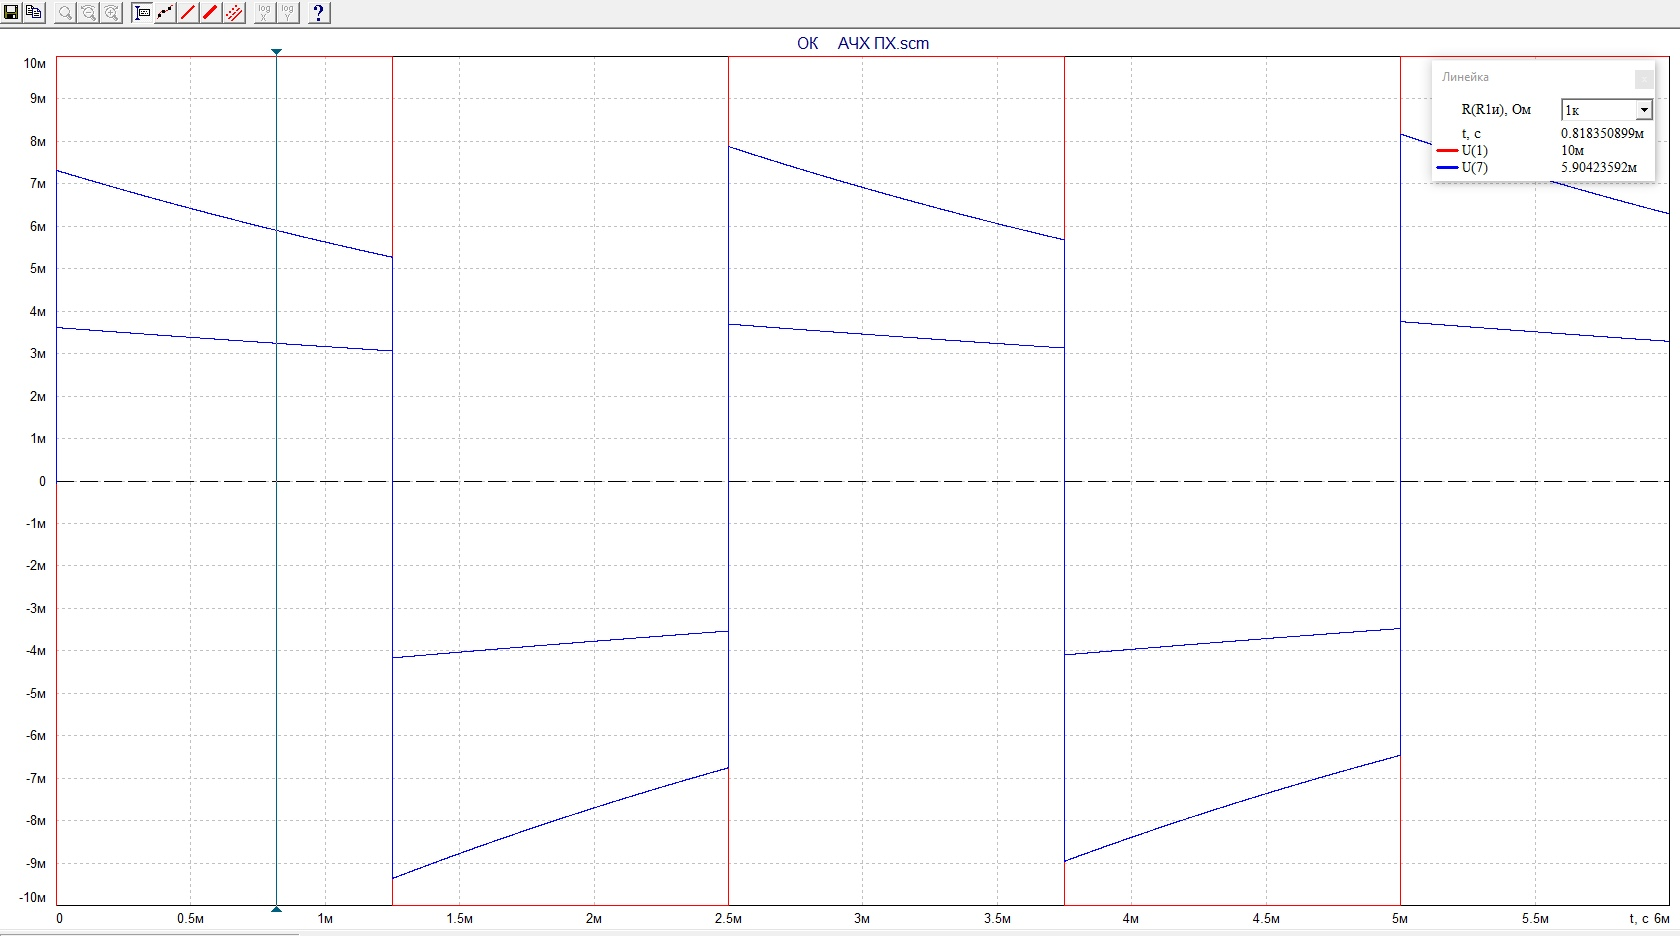
\includegraphics[scale=0.3]{5.4.jpg}
    \end{center}

    ПФ при f = 400Гц, $R_2$ = 3.6кОм 

    \textbf{Выводы по пункту 5:}
    \vspace{-6ex}
    \begin{singlespace}
        \begin{itemize}
           \item Увеличение $R_1$ уменьшает измеренный спад вершины импульса и увеличивает 
           $t_{\text{и}}$, а увеличение $R_2$ практически не оказывает эффекта на эти параметры 
           \item Увеличение $R_1$ уменьшает $K_{\text{скв}}$, а также сдвигает вниз по 
           частоте $f_{\text{н}}$ и $f_{\text{в}}$ и уменьшает рабочий диапазон частот. 
           Увеличение $R_2$ незначительно влияет на эти параметры.
        \end{itemize}
    \end{singlespace}
\end{document}